\documentclass[10pt]{article}
\usepackage[preprint]{tmlr}
% \usepackage{tmlr}            % anonymous submission version
\usepackage{amsmath,amssymb,amsthm}
\usepackage{booktabs}
\usepackage{graphicx}
\usepackage{hyperref}
\usepackage{url}
\usepackage{xcolor}
\usepackage{multirow}
%%%%% NEW MATH DEFINITIONS %%%%%

\usepackage{amsmath,amsfonts,bm}

% Mark sections of captions for referring to divisions of figures
\newcommand{\figleft}{{\em (Left)}}
\newcommand{\figcenter}{{\em (Center)}}
\newcommand{\figright}{{\em (Right)}}
\newcommand{\figtop}{{\em (Top)}}
\newcommand{\figbottom}{{\em (Bottom)}}
\newcommand{\captiona}{{\em (a)}}
\newcommand{\captionb}{{\em (b)}}
\newcommand{\captionc}{{\em (c)}}
\newcommand{\captiond}{{\em (d)}}

% Highlight a newly defined term
\newcommand{\newterm}[1]{{\bf #1}}


% Figure reference, lower-case.
\def\figref#1{figure~\ref{#1}}
% Figure reference, capital. For start of sentence
\def\Figref#1{Figure~\ref{#1}}
\def\twofigref#1#2{figures \ref{#1} and \ref{#2}}
\def\quadfigref#1#2#3#4{figures \ref{#1}, \ref{#2}, \ref{#3} and \ref{#4}}
% Section reference, lower-case.
\def\secref#1{section~\ref{#1}}
% Section reference, capital.
\def\Secref#1{Section~\ref{#1}}
% Reference to two sections.
\def\twosecrefs#1#2{sections \ref{#1} and \ref{#2}}
% Reference to three sections.
\def\secrefs#1#2#3{sections \ref{#1}, \ref{#2} and \ref{#3}}
% Reference to an equation, lower-case.
\def\eqref#1{equation~\ref{#1}}
% Reference to an equation, upper case
\def\Eqref#1{Equation~\ref{#1}}
% A raw reference to an equation---avoid using if possible
\def\plaineqref#1{\ref{#1}}
% Reference to a chapter, lower-case.
\def\chapref#1{chapter~\ref{#1}}
% Reference to an equation, upper case.
\def\Chapref#1{Chapter~\ref{#1}}
% Reference to a range of chapters
\def\rangechapref#1#2{chapters\ref{#1}--\ref{#2}}
% Reference to an algorithm, lower-case.
\def\algref#1{algorithm~\ref{#1}}
% Reference to an algorithm, upper case.
\def\Algref#1{Algorithm~\ref{#1}}
\def\twoalgref#1#2{algorithms \ref{#1} and \ref{#2}}
\def\Twoalgref#1#2{Algorithms \ref{#1} and \ref{#2}}
% Reference to a part, lower case
\def\partref#1{part~\ref{#1}}
% Reference to a part, upper case
\def\Partref#1{Part~\ref{#1}}
\def\twopartref#1#2{parts \ref{#1} and \ref{#2}}

\def\ceil#1{\lceil #1 \rceil}
\def\floor#1{\lfloor #1 \rfloor}
\def\1{\bm{1}}
\newcommand{\train}{\mathcal{D}}
\newcommand{\valid}{\mathcal{D_{\mathrm{valid}}}}
\newcommand{\test}{\mathcal{D_{\mathrm{test}}}}

\def\eps{{\epsilon}}


% Random variables
\def\reta{{\textnormal{$\eta$}}}
\def\ra{{\textnormal{a}}}
\def\rb{{\textnormal{b}}}
\def\rc{{\textnormal{c}}}
\def\rd{{\textnormal{d}}}
\def\re{{\textnormal{e}}}
\def\rf{{\textnormal{f}}}
\def\rg{{\textnormal{g}}}
\def\rh{{\textnormal{h}}}
\def\ri{{\textnormal{i}}}
\def\rj{{\textnormal{j}}}
\def\rk{{\textnormal{k}}}
\def\rl{{\textnormal{l}}}
% rm is already a command, just don't name any random variables m
\def\rn{{\textnormal{n}}}
\def\ro{{\textnormal{o}}}
\def\rp{{\textnormal{p}}}
\def\rq{{\textnormal{q}}}
\def\rr{{\textnormal{r}}}
\def\rs{{\textnormal{s}}}
\def\rt{{\textnormal{t}}}
\def\ru{{\textnormal{u}}}
\def\rv{{\textnormal{v}}}
\def\rw{{\textnormal{w}}}
\def\rx{{\textnormal{x}}}
\def\ry{{\textnormal{y}}}
\def\rz{{\textnormal{z}}}

% Random vectors
\def\rvepsilon{{\mathbf{\epsilon}}}
\def\rvtheta{{\mathbf{\theta}}}
\def\rva{{\mathbf{a}}}
\def\rvb{{\mathbf{b}}}
\def\rvc{{\mathbf{c}}}
\def\rvd{{\mathbf{d}}}
\def\rve{{\mathbf{e}}}
\def\rvf{{\mathbf{f}}}
\def\rvg{{\mathbf{g}}}
\def\rvh{{\mathbf{h}}}
\def\rvu{{\mathbf{i}}}
\def\rvj{{\mathbf{j}}}
\def\rvk{{\mathbf{k}}}
\def\rvl{{\mathbf{l}}}
\def\rvm{{\mathbf{m}}}
\def\rvn{{\mathbf{n}}}
\def\rvo{{\mathbf{o}}}
\def\rvp{{\mathbf{p}}}
\def\rvq{{\mathbf{q}}}
\def\rvr{{\mathbf{r}}}
\def\rvs{{\mathbf{s}}}
\def\rvt{{\mathbf{t}}}
\def\rvu{{\mathbf{u}}}
\def\rvv{{\mathbf{v}}}
\def\rvw{{\mathbf{w}}}
\def\rvx{{\mathbf{x}}}
\def\rvy{{\mathbf{y}}}
\def\rvz{{\mathbf{z}}}

% Elements of random vectors
\def\erva{{\textnormal{a}}}
\def\ervb{{\textnormal{b}}}
\def\ervc{{\textnormal{c}}}
\def\ervd{{\textnormal{d}}}
\def\erve{{\textnormal{e}}}
\def\ervf{{\textnormal{f}}}
\def\ervg{{\textnormal{g}}}
\def\ervh{{\textnormal{h}}}
\def\ervi{{\textnormal{i}}}
\def\ervj{{\textnormal{j}}}
\def\ervk{{\textnormal{k}}}
\def\ervl{{\textnormal{l}}}
\def\ervm{{\textnormal{m}}}
\def\ervn{{\textnormal{n}}}
\def\ervo{{\textnormal{o}}}
\def\ervp{{\textnormal{p}}}
\def\ervq{{\textnormal{q}}}
\def\ervr{{\textnormal{r}}}
\def\ervs{{\textnormal{s}}}
\def\ervt{{\textnormal{t}}}
\def\ervu{{\textnormal{u}}}
\def\ervv{{\textnormal{v}}}
\def\ervw{{\textnormal{w}}}
\def\ervx{{\textnormal{x}}}
\def\ervy{{\textnormal{y}}}
\def\ervz{{\textnormal{z}}}

% Random matrices
\def\rmA{{\mathbf{A}}}
\def\rmB{{\mathbf{B}}}
\def\rmC{{\mathbf{C}}}
\def\rmD{{\mathbf{D}}}
\def\rmE{{\mathbf{E}}}
\def\rmF{{\mathbf{F}}}
\def\rmG{{\mathbf{G}}}
\def\rmH{{\mathbf{H}}}
\def\rmI{{\mathbf{I}}}
\def\rmJ{{\mathbf{J}}}
\def\rmK{{\mathbf{K}}}
\def\rmL{{\mathbf{L}}}
\def\rmM{{\mathbf{M}}}
\def\rmN{{\mathbf{N}}}
\def\rmO{{\mathbf{O}}}
\def\rmP{{\mathbf{P}}}
\def\rmQ{{\mathbf{Q}}}
\def\rmR{{\mathbf{R}}}
\def\rmS{{\mathbf{S}}}
\def\rmT{{\mathbf{T}}}
\def\rmU{{\mathbf{U}}}
\def\rmV{{\mathbf{V}}}
\def\rmW{{\mathbf{W}}}
\def\rmX{{\mathbf{X}}}
\def\rmY{{\mathbf{Y}}}
\def\rmZ{{\mathbf{Z}}}

% Elements of random matrices
\def\ermA{{\textnormal{A}}}
\def\ermB{{\textnormal{B}}}
\def\ermC{{\textnormal{C}}}
\def\ermD{{\textnormal{D}}}
\def\ermE{{\textnormal{E}}}
\def\ermF{{\textnormal{F}}}
\def\ermG{{\textnormal{G}}}
\def\ermH{{\textnormal{H}}}
\def\ermI{{\textnormal{I}}}
\def\ermJ{{\textnormal{J}}}
\def\ermK{{\textnormal{K}}}
\def\ermL{{\textnormal{L}}}
\def\ermM{{\textnormal{M}}}
\def\ermN{{\textnormal{N}}}
\def\ermO{{\textnormal{O}}}
\def\ermP{{\textnormal{P}}}
\def\ermQ{{\textnormal{Q}}}
\def\ermR{{\textnormal{R}}}
\def\ermS{{\textnormal{S}}}
\def\ermT{{\textnormal{T}}}
\def\ermU{{\textnormal{U}}}
\def\ermV{{\textnormal{V}}}
\def\ermW{{\textnormal{W}}}
\def\ermX{{\textnormal{X}}}
\def\ermY{{\textnormal{Y}}}
\def\ermZ{{\textnormal{Z}}}

% Vectors
\def\vzero{{\bm{0}}}
\def\vone{{\bm{1}}}
\def\vmu{{\bm{\mu}}}
\def\vtheta{{\bm{\theta}}}
\def\va{{\bm{a}}}
\def\vb{{\bm{b}}}
\def\vc{{\bm{c}}}
\def\vd{{\bm{d}}}
\def\ve{{\bm{e}}}
\def\vf{{\bm{f}}}
\def\vg{{\bm{g}}}
\def\vh{{\bm{h}}}
\def\vi{{\bm{i}}}
\def\vj{{\bm{j}}}
\def\vk{{\bm{k}}}
\def\vl{{\bm{l}}}
\def\vm{{\bm{m}}}
\def\vn{{\bm{n}}}
\def\vo{{\bm{o}}}
\def\vp{{\bm{p}}}
\def\vq{{\bm{q}}}
\def\vr{{\bm{r}}}
\def\vs{{\bm{s}}}
\def\vt{{\bm{t}}}
\def\vu{{\bm{u}}}
\def\vv{{\bm{v}}}
\def\vw{{\bm{w}}}
\def\vx{{\bm{x}}}
\def\vy{{\bm{y}}}
\def\vz{{\bm{z}}}

% Elements of vectors
\def\evalpha{{\alpha}}
\def\evbeta{{\beta}}
\def\evepsilon{{\epsilon}}
\def\evlambda{{\lambda}}
\def\evomega{{\omega}}
\def\evmu{{\mu}}
\def\evpsi{{\psi}}
\def\evsigma{{\sigma}}
\def\evtheta{{\theta}}
\def\eva{{a}}
\def\evb{{b}}
\def\evc{{c}}
\def\evd{{d}}
\def\eve{{e}}
\def\evf{{f}}
\def\evg{{g}}
\def\evh{{h}}
\def\evi{{i}}
\def\evj{{j}}
\def\evk{{k}}
\def\evl{{l}}
\def\evm{{m}}
\def\evn{{n}}
\def\evo{{o}}
\def\evp{{p}}
\def\evq{{q}}
\def\evr{{r}}
\def\evs{{s}}
\def\evt{{t}}
\def\evu{{u}}
\def\evv{{v}}
\def\evw{{w}}
\def\evx{{x}}
\def\evy{{y}}
\def\evz{{z}}

% Matrix
\def\mA{{\bm{A}}}
\def\mB{{\bm{B}}}
\def\mC{{\bm{C}}}
\def\mD{{\bm{D}}}
\def\mE{{\bm{E}}}
\def\mF{{\bm{F}}}
\def\mG{{\bm{G}}}
\def\mH{{\bm{H}}}
\def\mI{{\bm{I}}}
\def\mJ{{\bm{J}}}
\def\mK{{\bm{K}}}
\def\mL{{\bm{L}}}
\def\mM{{\bm{M}}}
\def\mN{{\bm{N}}}
\def\mO{{\bm{O}}}
\def\mP{{\bm{P}}}
\def\mQ{{\bm{Q}}}
\def\mR{{\bm{R}}}
\def\mS{{\bm{S}}}
\def\mT{{\bm{T}}}
\def\mU{{\bm{U}}}
\def\mV{{\bm{V}}}
\def\mW{{\bm{W}}}
\def\mX{{\bm{X}}}
\def\mY{{\bm{Y}}}
\def\mZ{{\bm{Z}}}
\def\mBeta{{\bm{\beta}}}
\def\mPhi{{\bm{\Phi}}}
\def\mLambda{{\bm{\Lambda}}}
\def\mSigma{{\bm{\Sigma}}}

% Tensor
\DeclareMathAlphabet{\mathsfit}{\encodingdefault}{\sfdefault}{m}{sl}
\SetMathAlphabet{\mathsfit}{bold}{\encodingdefault}{\sfdefault}{bx}{n}
\newcommand{\tens}[1]{\bm{\mathsfit{#1}}}
\def\tA{{\tens{A}}}
\def\tB{{\tens{B}}}
\def\tC{{\tens{C}}}
\def\tD{{\tens{D}}}
\def\tE{{\tens{E}}}
\def\tF{{\tens{F}}}
\def\tG{{\tens{G}}}
\def\tH{{\tens{H}}}
\def\tI{{\tens{I}}}
\def\tJ{{\tens{J}}}
\def\tK{{\tens{K}}}
\def\tL{{\tens{L}}}
\def\tM{{\tens{M}}}
\def\tN{{\tens{N}}}
\def\tO{{\tens{O}}}
\def\tP{{\tens{P}}}
\def\tQ{{\tens{Q}}}
\def\tR{{\tens{R}}}
\def\tS{{\tens{S}}}
\def\tT{{\tens{T}}}
\def\tU{{\tens{U}}}
\def\tV{{\tens{V}}}
\def\tW{{\tens{W}}}
\def\tX{{\tens{X}}}
\def\tY{{\tens{Y}}}
\def\tZ{{\tens{Z}}}


% Graph
\def\gA{{\mathcal{A}}}
\def\gB{{\mathcal{B}}}
\def\gC{{\mathcal{C}}}
\def\gD{{\mathcal{D}}}
\def\gE{{\mathcal{E}}}
\def\gF{{\mathcal{F}}}
\def\gG{{\mathcal{G}}}
\def\gH{{\mathcal{H}}}
\def\gI{{\mathcal{I}}}
\def\gJ{{\mathcal{J}}}
\def\gK{{\mathcal{K}}}
\def\gL{{\mathcal{L}}}
\def\gM{{\mathcal{M}}}
\def\gN{{\mathcal{N}}}
\def\gO{{\mathcal{O}}}
\def\gP{{\mathcal{P}}}
\def\gQ{{\mathcal{Q}}}
\def\gR{{\mathcal{R}}}
\def\gS{{\mathcal{S}}}
\def\gT{{\mathcal{T}}}
\def\gU{{\mathcal{U}}}
\def\gV{{\mathcal{V}}}
\def\gW{{\mathcal{W}}}
\def\gX{{\mathcal{X}}}
\def\gY{{\mathcal{Y}}}
\def\gZ{{\mathcal{Z}}}

% Sets
\def\sA{{\mathbb{A}}}
\def\sB{{\mathbb{B}}}
\def\sC{{\mathbb{C}}}
\def\sD{{\mathbb{D}}}
% Don't use a set called E, because this would be the same as our symbol
% for expectation.
\def\sF{{\mathbb{F}}}
\def\sG{{\mathbb{G}}}
\def\sH{{\mathbb{H}}}
\def\sI{{\mathbb{I}}}
\def\sJ{{\mathbb{J}}}
\def\sK{{\mathbb{K}}}
\def\sL{{\mathbb{L}}}
\def\sM{{\mathbb{M}}}
\def\sN{{\mathbb{N}}}
\def\sO{{\mathbb{O}}}
\def\sP{{\mathbb{P}}}
\def\sQ{{\mathbb{Q}}}
\def\sR{{\mathbb{R}}}
\def\sS{{\mathbb{S}}}
\def\sT{{\mathbb{T}}}
\def\sU{{\mathbb{U}}}
\def\sV{{\mathbb{V}}}
\def\sW{{\mathbb{W}}}
\def\sX{{\mathbb{X}}}
\def\sY{{\mathbb{Y}}}
\def\sZ{{\mathbb{Z}}}

% Entries of a matrix
\def\emLambda{{\Lambda}}
\def\emA{{A}}
\def\emB{{B}}
\def\emC{{C}}
\def\emD{{D}}
\def\emE{{E}}
\def\emF{{F}}
\def\emG{{G}}
\def\emH{{H}}
\def\emI{{I}}
\def\emJ{{J}}
\def\emK{{K}}
\def\emL{{L}}
\def\emM{{M}}
\def\emN{{N}}
\def\emO{{O}}
\def\emP{{P}}
\def\emQ{{Q}}
\def\emR{{R}}
\def\emS{{S}}
\def\emT{{T}}
\def\emU{{U}}
\def\emV{{V}}
\def\emW{{W}}
\def\emX{{X}}
\def\emY{{Y}}
\def\emZ{{Z}}
\def\emSigma{{\Sigma}}

% entries of a tensor
% Same font as tensor, without \bm wrapper
\newcommand{\etens}[1]{\mathsfit{#1}}
\def\etLambda{{\etens{\Lambda}}}
\def\etA{{\etens{A}}}
\def\etB{{\etens{B}}}
\def\etC{{\etens{C}}}
\def\etD{{\etens{D}}}
\def\etE{{\etens{E}}}
\def\etF{{\etens{F}}}
\def\etG{{\etens{G}}}
\def\etH{{\etens{H}}}
\def\etI{{\etens{I}}}
\def\etJ{{\etens{J}}}
\def\etK{{\etens{K}}}
\def\etL{{\etens{L}}}
\def\etM{{\etens{M}}}
\def\etN{{\etens{N}}}
\def\etO{{\etens{O}}}
\def\etP{{\etens{P}}}
\def\etQ{{\etens{Q}}}
\def\etR{{\etens{R}}}
\def\etS{{\etens{S}}}
\def\etT{{\etens{T}}}
\def\etU{{\etens{U}}}
\def\etV{{\etens{V}}}
\def\etW{{\etens{W}}}
\def\etX{{\etens{X}}}
\def\etY{{\etens{Y}}}
\def\etZ{{\etens{Z}}}

% The true underlying data generating distribution
\newcommand{\pdata}{p_{\rm{data}}}
% The empirical distribution defined by the training set
\newcommand{\ptrain}{\hat{p}_{\rm{data}}}
\newcommand{\Ptrain}{\hat{P}_{\rm{data}}}
% The model distribution
\newcommand{\pmodel}{p_{\rm{model}}}
\newcommand{\Pmodel}{P_{\rm{model}}}
\newcommand{\ptildemodel}{\tilde{p}_{\rm{model}}}
% Stochastic autoencoder distributions
\newcommand{\pencode}{p_{\rm{encoder}}}
\newcommand{\pdecode}{p_{\rm{decoder}}}
\newcommand{\precons}{p_{\rm{reconstruct}}}

\newcommand{\laplace}{\mathrm{Laplace}} % Laplace distribution

\newcommand{\E}{\mathbb{E}}
\newcommand{\Ls}{\mathcal{L}}
\newcommand{\R}{\mathbb{R}}
\newcommand{\emp}{\tilde{p}}
\newcommand{\lr}{\alpha}
\newcommand{\reg}{\lambda}
\newcommand{\rect}{\mathrm{rectifier}}
\newcommand{\softmax}{\mathrm{softmax}}
\newcommand{\sigmoid}{\sigma}
\newcommand{\softplus}{\zeta}
\newcommand{\KL}{D_{\mathrm{KL}}}
\newcommand{\Var}{\mathrm{Var}}
\newcommand{\standarderror}{\mathrm{SE}}
\newcommand{\Cov}{\mathrm{Cov}}
% Wolfram Mathworld says $L^2$ is for function spaces and $\ell^2$ is for vectors
% But then they seem to use $L^2$ for vectors throughout the site, and so does
% wikipedia.
\newcommand{\normlzero}{L^0}
\newcommand{\normlone}{L^1}
\newcommand{\normltwo}{L^2}
\newcommand{\normlp}{L^p}
\newcommand{\normmax}{L^\infty}

\newcommand{\parents}{Pa} % See usage in notation.tex. Chosen to match Daphne's book.

\DeclareMathOperator*{\argmax}{arg\,max}
\DeclareMathOperator*{\argmin}{arg\,min}

\DeclareMathOperator{\sign}{sign}
\DeclareMathOperator{\Tr}{Tr}
\let\ab\allowbreak


\newtheorem{proposition}{Proposition}
\newtheorem{definition}{Definition}

\title{Capacity or Classifier? What Expansion Triggers Detect in\\Task-Free Continual Adapter Learning, and When Expansion Pays}
\author{Anonymous authors}

\newcommand{\ls}{\textsc{LabelSurprise}}
\newcommand{\pend}[1]{\textcolor{red}{[#1]}}

\begin{document}
\maketitle

\begin{abstract}
Dynamic-expansion continual learners add an adapter when a trigger---a loss spike, a representation shift, a prospective-forgetting estimate, or the utility of a fresh module---signals that existing capacity is inadequate. We ask what these triggers detect and when expanding is worth it. At the arrival of labels that the current module's classifier has never trained on, the excess loss depends on the input only through the old labels' logits, so loss-based triggers and one-step fresh-module utility are \emph{classifier-novelty} detectors. In a pre-registered study (ten text streams, three held out; DistilBERT, a held-out BERT backbone and ViT-B/16), every loss-spike and fresh-utility expansion in class-incremental streams fell at package-level label novelty. We then measure the value of expansion directly against two references, a single adapter that keeps learning and first-session adaptation. When the learner keeps exemplars from which its classifier statistics are refreshed, oracle expansion at the true boundaries costs 7--11 points in class-incremental streams relative to a single adapter, is neutral under domain shift and mixed under concept drift, although it beats first-session adaptation, the reference used in self-expansion ablations. When the learner is exemplar-free, so that a training adapter's prototypes go stale, the sign flips: \pend{EXT2}. Refreshing stale prototypes without exemplars by semantic drift compensation \pend{EXT4}, and the same interaction appears inside the official implementation of a published self-expanding method (SEMA) \pend{SEMA}. Expansion at classifier novelty is therefore a remedy for stale classifier statistics rather than for missing capacity, and its value depends on whether those statistics can be refreshed. We recommend that expansion triggers be evaluated by the measured value of expansion against both reference points, not by boundary precision.
\end{abstract}

\section{Introduction}

Parameter-efficient continual learning commonly grows a pool of adapters around a frozen pre-trained model \citep{zhou2024ease,wang2025sema,wei2025onlinelora}. When task identities are unavailable---the task-free setting \citep{aljundi2019taskfree}---the learner must itself decide \emph{when} to allocate a new module. Published decision rules monitor training-loss spikes or plateaus \citep{wei2025onlinelora,tathe2026lace}, distribution-shift descriptors of intermediate representations \citep{wang2025sema}, prospective forgetting after a virtual update \citep{julian2025cable}, or the hindrance a new task places on forward learning \citep{feng2024lw2g}. These signals are usually validated by \emph{boundary precision}---whether expansions coincide with the hidden task boundaries of a benchmark---or by ablations against a model that adapts only on the first task.

Boundary precision and the \emph{value} of expansion are different quantities. Most boundaries in standard benchmarks are class-incremental: new labels arrive with new inputs. A learner whose classifier can grow new output rows, on top of a pre-trained representation that already separates the new classes reasonably well, may need no new adapter at all. Whether a new adapter is nevertheless useful can depend on something other than capacity: in exemplar-free learners, class prototypes recorded under an adapter that keeps training become stale \citep{yu2020sdc}, and freezing that adapter---which is what expansion does---keeps them valid.

This paper asks what common expansion triggers detect, and when what they detect warrants expansion. Our contributions are:
\begin{enumerate}
\item \textbf{A diagnostic.} We show (Proposition~\ref{prop:novelty}) that at a package-level label-novelty event the excess loss of an existing module depends on the input only through its old-label logits, so loss-spike triggers and one-step fresh-module utility respond to classifier novelty, not to representational inadequacy. Empirically, every loss-spike and fresh-utility expansion in our class-incremental streams falls at such an event.
\item \textbf{A value-of-expansion protocol.} We measure the value of expansion with oracle expansion at the true boundaries and count-matched random timing, against two references---a single adapter that keeps learning with the same memory budget, and first-session adaptation \citep{panos2023fsa,zhou2024aper}---with trigger thresholds calibrated on shift-free nulls rather than tuned on outcomes.
\item \textbf{A regime map.} In the exemplar-based regime, expansion hurts in class-incremental streams yet beats first-session adaptation, so the conclusion of a self-expansion ablation depends on its reference point. In the exemplar-free regime the sign flips \pend{EXT2}. Two mechanism tests support stale classifier statistics as the cause: the flip appears within identical training trajectories when only the prototype rule changes, and exemplar-free drift compensation \pend{EXT4}. The interaction replicates in vision (ViT-B/16, CIFAR-100, ImageNet-R) and inside SEMA's official implementation \pend{SEMA}.
\item \textbf{A label-conditional detector, and why detection is not enough.} \ls{} compares each example's loss with the recent loss of its own label and ignores labels without history. It never expands at class arrivals and fires when established labels change, but its expansions help only where expansion helps.
\end{enumerate}
The study was pre-registered with frozen code hashes in four stages, uses the seed as the unit of analysis, and reports every failed hypothesis. We do not propose a method that competes with the state of the art; our learner is deliberately simple so that the expansion decision is the only moving part.

\section{Related work}

\paragraph{Expansion in continual learning.} Architectural approaches add capacity per task \citep{rusu2016pnn,yoon2018den} or on demand in task-free streams \citep{lee2020cndpm,ye2023sedem}. With pre-trained models, adapter pools are expanded per task \citep{zhou2024ease} or when a shift is detected: SEMA uses autoencoder-based representation descriptors \citep{wang2025sema}, Online-LoRA monitors loss plateaus \citep{wei2025onlinelora}, LACE expands on loss spikes relative to a recent-loss baseline \citep{tathe2026lace}, CABLE scores prospective forgetting after a virtual update \citep{julian2025cable}, and LW2G learns whether to grow from a hindrance metric \citep{feng2024lw2g}. These signals are validated by boundary precision---LACE reports that all of its expansions fall at domain boundaries---or by ablations that remove expansion while keeping first-session adaptation, as in SEMA. We stylise the signals of these families inside one learner, evaluate a LACE-style rule with its published threshold, and run SEMA's own code with the expansion decision varied.

\paragraph{Reference points for pre-trained-model continual learning.} Adapting a pre-trained model on the first session and freezing it is a strong replay-free baseline \citep{panos2023fsa,zhou2024aper}, and prototype classifiers on pre-trained features are strong in general \citep{rebuffi2017icarl,mai2021scr,mcdonnell2023ranpac}. Continual fine-tuning of a single model is competitive when representation learning is slowed and the classifier is re-aligned \citep{zhang2023slca}. In exemplar-free learning, the features of old classes drift while the model trains; semantic drift compensation estimates this drift from current data \citep{yu2020sdc,gomezvilla2024ldc}, and SSIAT keeps a single shared adapter with semantic-shift compensation \citep{tan2024ssiat}. We use these as the two references of the value-of-expansion protocol and as an exemplar-free alternative to expansion.

\paragraph{Classifier effects in class-incremental learning.} Output-layer bias toward recent classes is well documented \citep{wu2019bic,hou2019lucir,caccia2022ace}, and the factorisation of class-incremental prediction into task-identity and within-task prediction is established \citep{kim2022theoretical}. We use the corresponding loss identity as a diagnostic of expansion triggers; the identity itself is not new.

\paragraph{Drift and novelty detection in streams.} Error-rate drift detectors \citep{page1954cusum,gama2004ddm,bifet2007adwin} and novel-class detection under concept drift \citep{masud2011novel} distinguish concept change from class emergence in classical stream mining, and class-specific monitoring avoids the masking of drift by class-prior changes \citep{wang2013ddmoci}. \ls{} transfers this label-conditional view to the expansion decision.

\section{Setting and learner}
\label{sec:setting}

\paragraph{Stream.} A task-free learner observes batches $(\mathbf{x}_t,\mathbf{y}_t)$, $t=1,\dots,T$, of 16 labelled examples. Segment identities are evaluation metadata and are never shown to the learner, except by the oracle reference policy.

\paragraph{Packages.} A frozen encoder $f$ (DistilBERT \citep{sanh2019distilbert}; BERT-base \citep{devlin2019bert} as held-out backbone; ViT-B/16 pre-trained on ImageNet-21k \citep{dosovitskiy2021vit} for vision) is shared. A package $k$ consists of LoRA factors \citep{hu2022lora} on query/value projections (rank 8) and a linear head over the global label space. Only the newest package trains; earlier packages are frozen, as in expand-and-freeze adapter pools \citep{zhou2024ease,wang2025sema}. A new package starts from zero-output LoRA and a zero head.

\paragraph{Training.} For every incoming batch the newest package takes two AdamW steps on the batch plus, in the exemplar-based regime, 16 items replayed from its own memory \citep{chaudhry2019tiny}, with cross-entropy over the labels observed so far.

\paragraph{Memory.} A single global reservoir \citep{vitter1985reservoir} of 512 examples is shared by the whole pool, so expansion never increases the memory budget.

\paragraph{Two regimes of classifier statistics.} Predictions use cosine prototypes; class scores are averaged over packages (equivalently, nearest-class-mean on the normalised concatenation of package features, as in EASE \citep{zhou2024ease}). In the \emph{exemplar-based} regime, prototypes are recomputed from memory under each package at prediction time, so they always match the current features. In the \emph{exemplar-free} regime (no replay, as in APER, EASE and SEMA), each package accumulates class means of features computed when the examples were observed and never recomputes them; a package spawned after a class was observed holds no prototype for it. Prototypes of a package that keeps training therefore go stale, while those of a frozen package stay valid. (Task-based methods compute prototypes once a task has ended; a task-free learner has no task end, so prototypes accumulate online. Drift compensation, Section~\ref{sec:triggers}, is the standard remedy for the resulting staleness.) Every exemplar-free run also reports the exemplar-based rule on the identical trajectory, which isolates the refresh factor.

\paragraph{Learner competence.} A single package reaches 85\% on the BANKING77 recurrence stream versus 65\% for training-free frozen-feature prototypes (Table~\ref{tab:main}). An earlier version of this project used a learner that reached only 16\%---below the training-free baseline---and we discarded its accuracy comparisons (Appendix~\ref{app:history}).

\section{What a loss signal measures at a label-novelty event}
\label{sec:mechanism}

Let $S$ be the labels that may be predicted, partitioned into labels $O$ already trained \emph{by the current package} and labels $N$ in the current batch whose head rows in that package have never been updated. $N$ contains labels new to the stream, but also labels seen before the package was created: in an expand-and-freeze pool, a returning label group is new to the package spawned since it was last seen. We call both \emph{package-level label novelty}. For an example with label $y$ in group $G(y)\in\{O,N\}$,
\begin{equation}
\ell(x,y) = \underbrace{-\log \textstyle\sum_{c\in G(y)} p(c\mid x)}_{\text{label-group term}}\;\underbrace{-\;\log p\big(y \mid x, G(y)\big)}_{\text{within-group term}} .
\label{eq:decomp}
\end{equation}

\begin{proposition}
\label{prop:novelty}
Suppose the head rows of labels in $N$ have never been updated and are zero, so $z_c(x)=0$ for $c\in N$. For $y\in N$ the loss of an existing package is
\[
\ell(x,y) = \log|N| \;+\; \log\Big(1+\tfrac{1}{|N|}\textstyle\sum_{o\in O} e^{z_o(x)}\Big),
\]
where the first term is the within-group term and the second is the label-group term. A fresh package with a zero head incurs $\log(|N|+|O|)$. Hence the advantage of the fresh package before any update (reuse loss minus fresh loss) is $\log\big((|N|+\sum_{o}e^{z_o(x)})/(|N|+|O|)\big)$, which is positive whenever the mean of $e^{z_o(x)}$ over old labels exceeds one, and which depends on $x$ only through the old-label logits.
\end{proposition}
\begin{proof}
With $z_c=0$ for $c\in N$, $p(y\mid x)=1/(|N|+\sum_o e^{z_o})$ and $p(y\mid x,N)=1/|N|$; the identity follows from \eqref{eq:decomp}. A zero head assigns $1/|S|$ to every label.
\end{proof}

The proposition is elementary, but its consequence for expansion triggers is direct. A loss-spike detector at a class arrival measures how confidently the old head predicts old labels; a fresh-versus-reuse utility comparison before or shortly after one update rewards discarding that confident head. Neither asks whether the representation can separate the new labels---a question that a growing head and a prototype classifier answer without new adapter capacity. The label-group term is 36--52\% of the boundary loss in our class-incremental streams even after several steps of learning (Figure~\ref{fig:mechanism}).

\begin{figure}[t]
\centering
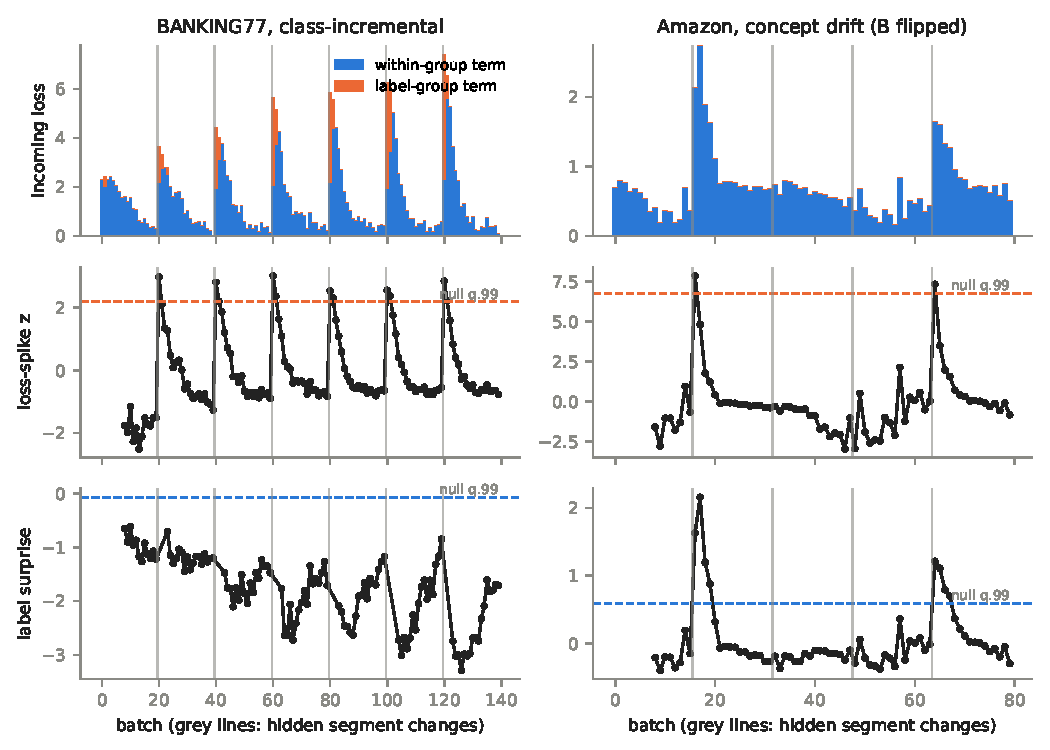
\includegraphics[width=\linewidth]{figures/mechanism.pdf}
\caption{Per-batch statistics of a single package on a class-incremental stream (left) and a concept-drift stream (right); development seed 2026. Top: incoming loss split as in \eqref{eq:decomp}. Middle: loss-spike $z$-score. Bottom: \ls{}. Dashed: null-calibrated thresholds ($q=0.99$). The loss spike crosses its threshold at every class arrival; \ls{} stays below its threshold under class arrivals and crosses it when established labels flip.}
\label{fig:mechanism}
\end{figure}

\subsection{A label-conditional alternative}
\label{sec:surprise}
If label novelty is to be absorbed by the classifier, expansion should respond to evidence that an \emph{established} label's mapping has changed. Let $B_y$ be the mean of the last 20 batch-mean losses of label $y$ under the current package.
\begin{definition}[\ls]
For a batch, $\mathrm{LS} = \frac{1}{|\mathcal{E}|}\sum_{i\in\mathcal{E}} \big(\ell(x_i,y_i) - B_{y_i}\big)$, where $\mathcal{E}$ contains the examples whose label has at least three prior batch-loss records under the current package. LS is undefined (cannot trigger) if $|\mathcal{E}|<4$.
\end{definition}
Newly introduced labels are excluded by construction, and while a label is being learned its loss falls, so LS is typically negative under class arrivals. Under concept drift, an established label's loss rises above its own history. LS is an error-based drift statistic \citep{gama2004ddm} computed per label. Two earlier variants failed during development (Appendix~\ref{app:history}).

\section{Triggers, references and protocol}
\label{sec:triggers}

\paragraph{Trigger statistics.} All triggers are computed on the newest package before it trains on the incoming batch. \textsc{LabelNovel}: fraction of batch labels never observed (a trivial reference). \textsc{LossZ}: $z$-score of the incoming loss against a 20-batch window (loss-spike triggers; \citealp{tathe2026lace,wei2025onlinelora}). \textsc{ReprZ}: $z$-score of a label-free diagonal-Mahalanobis feature distance (distribution-shift descriptors; \citealp{wang2025sema}). \textsc{InterfLogit}: increase in protected-memory cross-entropy after a virtual update (prospective forgetting; \citealp{julian2025cable}). \textsc{FreshUtil}: cross-fitted query-loss advantage of a fresh package over updating the current one after one virtual update (counterfactual utility; Appendix~\ref{app:cau}). Two further statistics, \textsc{InterfProto} and \textsc{ConflictZ}, are failed development proposals reported for completeness, and \ls{} is defined above. Virtual updates use exact snapshot/restore of parameters, optimiser moments and random states; a test verifies bitwise restoration.

\paragraph{Decision rule and calibration.} After the newest package has at least eight updates, a trigger spawns when its statistic exceeds its threshold on two consecutive batches; values in alarm are not added to baseline windows. Each threshold is the $0.99$-quantile of the statistic on an i.i.d.-shuffled version of the same stream (same examples, no shift) under the same backbone and regime, using only the development seed. This equalises false-alarm rates across triggers and uses no outcome.

\paragraph{Streams.} Class-incremental (CIL): BANKING77 \citep{casanueva2020banking} class-group recurrence (A B A C B) and seven disjoint groups, CLINC150 \citep{larson2019clinc} (ten groups of 15), \emph{held-out} 20 Newsgroups \citep{lang1995newsweeder}, Split CIFAR-100 \citep{krizhevsky2009cifar} (ten groups of ten) and ImageNet-R \citep{hendrycks2021imagenetr} (ten groups of 20). Same-label domain shift (DIL): Amazon reviews \citep{keung2020marc} across domains, \emph{held-out} SST-2$\to$Yelp$\to$tweets$\to$IMDB \citep{socher2013sst,zhang2015charcnn,barbieri2020tweeteval,maas2011imdb}, and a BREEDS-style \citep{santurkar2021breeds} CIFAR-100 superclass stream in which domain $d$ contains the $d$-th subclass of every superclass. Concept drift: the Amazon and sentiment streams with some domains' labels flipped, the CIFAR superclass stream with two domains relabelled, and a natural label-semantics stream of TweetEval tasks over the same tweet population. Development examples come from training splits only.

\paragraph{Policies.} \emph{Frozen}: training-free prototypes. \emph{Single}: one package throughout. \emph{First-segment}: one package trained on the first segment only, then frozen, while memory and prototypes keep updating (first-session adaptation). \emph{Oracle}: spawn at every true segment change. \emph{Random}: the oracle's number of spawns at uniformly random steps. \emph{Triggers}: the statistics above.

\paragraph{Exemplar-free refresh.} Semantic drift compensation (SDC; \citealp{yu2020sdc}) moves each stored prototype $\mu_c$ of the training package by the kernel-weighted mean drift of the current batch, $\Delta_c=\sum_i w_{ic}(z_i^{\text{new}}-z_i^{\text{old}})/\sum_i w_{ic}$ with $w_{ic}=\exp(-\|z_i^{\text{old}}-\mu_c\|^2/2\sigma^2)$, on normalised embeddings with the published $\sigma=0.3$. We apply it after every update, because a task-free stream has no tasks. SDC changes no training computation and is reported as a further prototype rule on the same trajectories.

\paragraph{Statistics and pre-registration.} The study was pre-registered in four stages before any confirmation run of each stage (repository files \texttt{notes/tmlr\_*prereg.md}, with code hashes): the primary text study (seeds 2027--2036; BERT 2027--2031); a vision, baseline-dependence and natural-drift extension (vision seeds 2027--2034); the exemplar-free regime (text 2027--2036, vision 2027--2034); and ImageNet-R plus drift compensation (5--6 seeds). Development used seed 2026 only. The seed is the unit of analysis. We report paired seed-level mean differences with 95\% $t$-intervals and two-sided Wilcoxon signed-rank tests, Holm-corrected within each hypothesis family; deviations are listed in Appendix~\ref{app:deviations}.

\section{Results}
\label{sec:results}

\begin{table}[t]\centering\caption{Placeholder.}\label{tab:main}\end{table}


\subsection{What the triggers detect}
\label{sec:res-detect}
\paragraph{Spawn attribution.} In the class-incremental streams without recurrence, every spawn of \textsc{LossZ} and \textsc{FreshUtil} fell within two batches after a batch containing a never-seen label (BANKING-CIL 55/55 and 55/55, CLINC 81/81 and 74/74, 20News \pend{n/n}, CIFAR-100 \pend{n/n}; pooled over seeds). On the recurrence stream BANKING-REC, only 45\% and 50\% did, so this pre-registered hypothesis failed there. When a label group returns, its labels are new to the package spawned since they were last seen, so Proposition~\ref{prop:novelty} applies; in an analysis declared after the failure, 100\% of \textsc{LossZ} and \textsc{FreshUtil} spawns in every class-incremental stream, BANKING-REC included, fell within two batches of package-level label novelty, against a base rate of 15--30\% of eligible batches.

\paragraph{A published threshold.} The LACE-style rule (loss above $2.5\times$ its recent mean; \citealp{tathe2026lace}) \pend{XL}.

\subsection{The value of expansion with exemplars}
\label{sec:res-exemplar}
\paragraph{Class-incremental: expansion hurts against a learner that keeps training\ldots} Oracle expansion at the true boundaries reduced final accuracy relative to a single package by 8.2 points on BANKING-REC, 11.4 on BANKING-CIL, 9.9 on CLINC and 7.1 on held-out 20~Newsgroups (every seed), and \pend{CIFAR} on CIFAR-100 with ViT-B/16. Count-matched random-timing expansion was also harmful, and on BANKING-REC less so than the oracle (79.2\% vs.\ 77.1\%).

\paragraph{\ldots but helps against first-session adaptation.} The same oracle pools beat the first-segment policy by 7.2, 5.5 and 6.9 points (every seed) and by 0.9 points on 20 Newsgroups (n.s.), \pend{CIFAR}. A self-expansion ablation of the usual form would therefore conclude that expansion helps, in exactly the setting where it costs 7--11 points against a single package that keeps learning, which itself beats first-session adaptation by 15--17 points (Figure~\ref{fig:regime}b).

\paragraph{Without rehearsal.} Removing replay from the training loss (memory still feeds the prototypes) reduced the harm of expansion: oracle$-$single was $-4.3$ on BANKING-REC (significant) and $-3.3$, $-0.6$, $-0.6$ on the other text CIL streams (n.s.), so our pre-registered prediction that the harm does not depend on rehearsal was mostly not supported. The difference-in-differences (without minus with replay) was $+3.9$ to $+9.3$ points in every stream (significant).

\paragraph{Domain shift and drift.} Under same-label domain shift, oracle expansion was within half a point of the single package. Under concept drift its value was mixed: $+1.9$ points [0.5, 3.3] on Amazon-DILCONF, $+0.8$ [$-2.1$, 3.8] (n.s.) on Amazon-CONFLICT, and $-17.5$ [$-20.5$, $-14.5$] on the held-out sentiment drift stream, the opposite of our pre-registered prediction. In that stream the domains are distinguishable, a single package trained with replay learns the domain-conditional mapping (82\% on the flipped Yelp segment at the end), and frozen packages trained on the unflipped mapping out-vote the correct package under prototype averaging (16\%). On the natural label-semantics stream, oracle expansion was $-0.8$ points \pend{final}. \pend{Vision DIL/drift; proto\_own.}

\subsection{The value of expansion without exemplars}
\label{sec:res-ef}
\pend{EXT2: R1 oracle vs single under proto\_ef per CIL stream; R2 within-run DiD; R3 loss\_z vs \ls{}; R4 oracle vs random; firstseg.}

\paragraph{Refreshing without exemplars.} \pend{EXT4: S1, S2; sigma sensitivity.}

\begin{figure}[t]
\centering
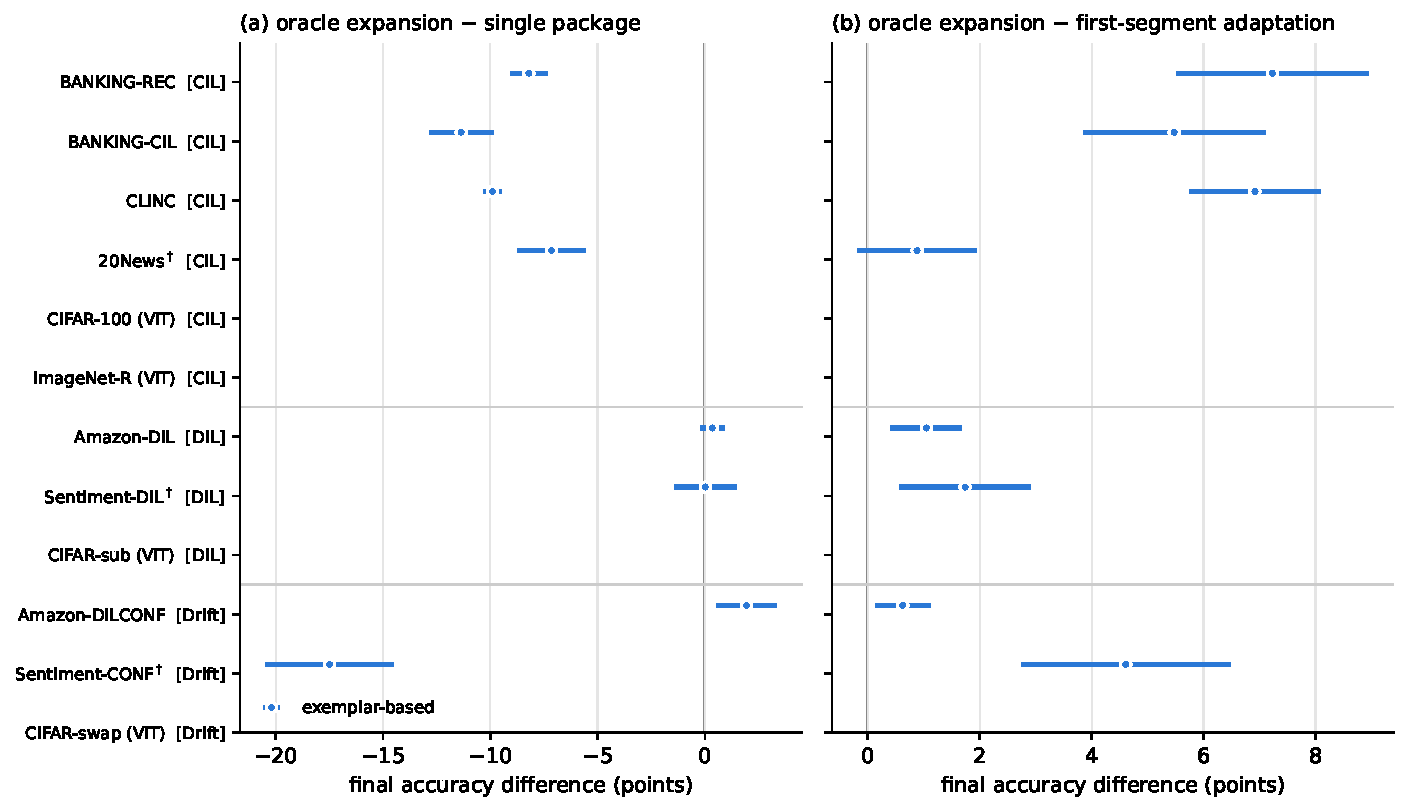
\includegraphics[width=\linewidth]{figures/regime.pdf}
\caption{Regime map. Paired seed-level difference in final accuracy (mean, 95\% $t$-interval) between oracle expansion and (a) a single package that keeps learning, (b) first-segment adaptation, with exemplar-refreshed prototypes (blue) and exemplar-free prototypes (orange). $^\dagger$held-out stream.}
\label{fig:regime}
\end{figure}

\subsection{A canonical benchmark and a published system}
\label{sec:res-external}
\paragraph{ImageNet-R.} \pend{EXT3: I1--I4.}

\paragraph{SEMA.} We ran SEMA's official implementation with its published CIFAR-100 configuration and varied only the expansion decision: the official rule; never expanding (adapters frozen after the first task, the reference of SEMA's own ablation); never expanding while the adapters keep training on every task; and expanding at every task. \pend{SEMA results: linear head / exemplar-free NCM vs exemplar NCM.}

\subsection{Closed-loop triggers and \ls{}}
\label{sec:res-closed}
Triggers that detect class boundaries spawned 3--5 packages per class-incremental stream and lost 4--10 points relative to the single package in the exemplar-based regime. \ls{} spawned essentially no package in any class-incremental or domain-shift stream, and so matched the single package (non-inferior in all seven), while on the drift streams it spawned 4--5 packages and tracked the oracle: $+2.1$ [0.9, 3.3] on Amazon-DILCONF, $+1.0$ (n.s.) on Amazon-CONFLICT and $-16.7$ on the held-out sentiment drift stream, where expansion itself is harmful. In the exemplar-free regime \pend{R3}. \pend{BERT, vision triggers.}

\section{Discussion and limitations}

\paragraph{What expansion buys.} \pend{Synthesis: expansion at classifier novelty freezes the features under which classifier statistics were recorded; it pays when those statistics cannot be refreshed and costs when they can. First-session adaptation, drift compensation and exemplar refresh are competing remedies.}

\paragraph{Scope.} Our encoders are small to medium, our streams are short (80--500 batches), and three of five drift streams use synthetic relabelling. Our triggers are stylised versions of published signals inside a common learner; the SEMA experiment checks one complete system, and we make no claim about reported benchmark numbers. The value of expansion also depends on the inference rule: routing each input to the package whose own prototypes fit best can recover part of the benefit of expansion under domain shift in vision (Appendix tables report all rules).

\paragraph{Calibration.} Thresholds are set on an i.i.d.-shuffled version of the same stream. This equalises false-alarm rates across triggers, which a comparison of triggers requires, but it is not available to a deployed learner. The conclusion that loss-type triggers fire at label arrivals does not depend on the threshold, since their AUROC for class arrivals is near one.

\paragraph{What \ls{} detects.} \ls{} responds to an increase in the loss of established labels. Concept drift produces this, but so does a within-label shift of $P(x\mid y)$, such as a new subpopulation under an existing superclass. It is therefore a detector of \emph{established-label degradation}, not of concept drift per se.

\paragraph{Training budget of the references.} Our first-segment policy trains for the same number of steps per batch as every other policy; SEMA and APER adapt for full epochs on the first task. The SEMA experiment uses SEMA's own budget.

\paragraph{Recommendations.} When an expansion trigger is proposed, its evaluation should include (i) the measured value of expansion in the evaluated regime against a single module that keeps learning with the same memory budget, and against first-session adaptation; (ii) a statement of whether classifier statistics are refreshed, since this decides the sign of the value of expansion at class arrivals; (iii) separation of label novelty from changes in established labels, since boundary precision on class-incremental benchmarks is achieved by label-novelty detection alone; and (iv) thresholds calibrated on shift-free nulls rather than tuned on outcomes.

\section{Conclusion}
\pend{TO BE WRITTEN AFTER CONFIRMATION.}

\paragraph{Use of AI assistants.} \pend{Statement: which parts were assisted by an AI coding/writing assistant; all claims, code and text were checked by the authors, who take full responsibility.}

\bibliography{refs}
\bibliographystyle{tmlr}

\appendix
\section{Development history and failed candidates}
\label{app:history}
This project began as the design of a task-free allocator (Appendix~\ref{app:cau}). Its learner took a single AdamW step per 16-example batch into a 77-way head and reached about 16\% final accuracy on the BANKING recurrence stream with label-free routing (22\% with a learned router), whereas training-free frozen-feature prototypes reached 71\% (logistic probe on frozen features: 86\%). We therefore discarded all of its accuracy comparisons and built the learner of Section~\ref{sec:setting}. All development of the new testbed used seed 2026 only:
\begin{enumerate}
\item \textsc{InterfProto} (head-equalised prospective interference) was our first proposal. On the seed-2026 shadow traces it did not detect concept drift (AUROC 0.54 and 0.22 on the two development drift streams).
\item \textsc{ConflictZ} v1 restricted the loss $z$-score to examples with previously observed labels. It detected class-incremental boundaries (AUROC 1.00) because labels observed one batch earlier are still untrained. v2 required labels to be first observed at least eight batches earlier; it still fired in class-incremental streams, because newly learned labels have higher loss than long-established ones. This motivated the label-conditional baseline of \ls{}.
\item The first closed-loop pilot added alarmed values to the $z$-score baseline windows, so a genuine spike inflated its own baseline. Excluding alarmed values applies identically to all $z$-type triggers.
\item A slower single learner (learning rate $10^{-4}$) did not reduce exemplar-free staleness in development (BANKING-CIL: 13.1\% vs.\ 26.2\% at $10^{-3}$) and was not carried into the confirmation.
\end{enumerate}
The thresholds, learner hyperparameters (learning rate $10^{-3}$, two steps per batch, replay 16, memory 512) and all trigger constants were fixed before the confirmation study.

\section{Pre-registration deviations}
\label{app:deviations}
\pend{List from notes: q=0.95 grid not run; BERT subset; H1 failure and post-hoc package-level analysis; A1 addendum; ext2 duplicate-launch note; reduced seeds in extensions 3--4.}

\section{Case study: an exact counterfactual allocator}
\label{app:cau}
Before this study, we developed and audited an allocator, CAU (counterfactual action utility), that compares an exact, optimiser-faithful one-step update of each existing package and of a fresh classifier-bearing package against a common no-update reference on cross-fitted query halves, subject to a separate protected-memory feasibility check, and spawns after two consecutive windows of positive fresh utility. On a BANKING77 class-group recurrence stream (A B A C B), CAU spawned exactly at the arrivals of the B and C label groups in all ten seed/order development trajectories. A \emph{head-only} variant---identical, except that LoRA outputs are held at zero and only the classifier trains---made identical allocation decisions in all ten trajectories. At the original spawn windows, about 87\% of the fresh-versus-best-reuse utility advantage was already present before the prospective update, i.e.\ it reflected the replacement of the old classifier rather than learning. These observations, made with the weaker learner of Appendix~\ref{app:history} and reported only for decisions, motivated Proposition~\ref{prop:novelty} and the present study.

\end{document}
